%
% $Id: cruise_listbox.tex,v 1.1 2001/08/03 20:17:16 klauko70 Exp $
%
\section{Kommando 'listbox'}
listbox LIST DEFAULT

\subsection{look and feel}
Das Bild zeigt die Listbox w�hrend der Interaktion.

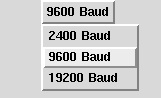
\includegraphics{cruise_listbox.eps}
\subsection{Verhalten w�hrend Interpretation}
Erzeugt eine Box mit dem Inhalt DEFAULT.

\subsection{Verhalten bei Interaktion}
Wird die Box mit dem Inhalt DEFAULT angeklickt, so �ffnet sich eine Auswahlliste
mit den Eintr�gen wie sie in der Liste LIST angegeben wurden. Der Benutzer kann
nun durch Auswahl eines Listeneintrags den neuen Wert bestimmen. Die
Auswahlliste verschwindet und anstelle des DEFAULT Wertes steht der neue
ausgew�hlte Wert.

\subsection{Beispiel}

\verb*|listbox {"2400 Baud" "9600 Baud" "19200 Baud"} "9600 Baud"|

erzeugt bei Interaktion eine Auswahlliste wie oben dargestellt.

